%Copyright 2014 Jean-Philippe Eisenbarth
%This program is free software: you can 
%redistribute it and/or modify it under the terms of the GNU General Public 
%License as published by the Free Software Foundation, either version 3 of the 
%License, or (at your option) any later version.
%This program is distributed in the hope that it will be useful,but WITHOUT ANY 
%WARRANTY; without even the implied warranty of MERCHANTABILITY or FITNESS FOR A 
%PARTICULAR PURPOSE. See the GNU General Public License for more details.
%You should have received a copy of the GNU General Public License along with 
%this program.  If not, see <http://www.gnu.org/licenses/>.

%Based on the code of Yiannis Lazarides
%http://tex.stackexchange.com/questions/42602/software-requirements-specification-with-latex
%http://tex.stackexchange.com/users/963/yiannis-lazarides
%Also based on the template of Karl E. Wiegers
%http://www.se.rit.edu/~emUmbrelload/teaching/slides/srs_template_sep14.pdf
%http://karlwiegers.com
\documentclass{scrreprt}
\usepackage{booktabs}
\usepackage{listings}
\usepackage{underscore}
\usepackage[bookmarks=true]{hyperref}
\usepackage[utf8]{inputenc}
\usepackage[english]{babel}
\hypersetup{
%    bookmarks=false,    % show bookmarks bar?
%    pdftitle={Software Requirement Specification},    % title
%    pdfauthor={Jean-Philippe Eisenbarth},                     % author
%    pdfsubject={TeX and LaTeX},                        % subject of the document
%    pdfkeywords={TeX, LaTeX, graphics, images}, % list of keywords
    colorlinks=true,       % false: boxed links; true: colored links
    linkcolor=blue,       % color of internal links
    citecolor=black,       % color of links to bibliography
    filecolor=black,        % color of file links
    urlcolor=blue% color of external links
%    linktoc=page            % only page is linked
}%
\def\myversion{1.0.0 }
\date{}
%\title
\usepackage{hyperref}
\usepackage{graphicx}
\begin{document}
\thispagestyle{empty}
\begin{flushright}
    \rule{16cm}{5pt}\vskip1cm
    \bfseries{
        \Huge{SOFTWARE REQUIREMENTS\\ SPECIFICATION}\\
        \vspace{1.9cm}
        for\\
        \vspace{1.9cm}
        Student Auditorium Management System (SAMS)\\
        \vspace{1.9cm}
        Prepared by \\
        Aaditya Agrawal (19CS10003)\\
        Debanjan Saha (19CS30014) \\
        Deep Majumder (19CS30015) \\ 
        \vspace{1.9cm}
        \today\\
}
\end{flushright}

\tableofcontents


\chapter*{Revision History}

\begin{center}
    \begin{tabular}{|c|c|c|c|}
        \hline
	    Name & Date & Reason For Changes & Version\\
        \hline
	     &  &  & \\
        \hline
    \end{tabular}
\end{center}

\chapter{Introduction}

\section{Purpose}
This document is to define the functional and non-functional requirements of the Student Auditorium Management System (SAMS). This software consists of a back-end API server and a front-end application, which together allow for efficiently managing shows, selling and refunding tickets and maintaining a balance sheet.

\section{Document Conventions}

Following definitions and abbreviations are used in this document:
\begin{enumerate}
	\item SAMS: Students' Auditorium Management System
	\item SM: Show Manager
	\item SP: Sales Person
	\item AC: Accounts Clerk
	\item User: User corresponds to either SM or AC or SP or customer.
\end{enumerate}

\section{Intended Audience and Reading Suggestions}

This document mainly focuses on the design analysis and requirement specifications for this software. Software developers, testers, documentation writers are always welcome to read this document. However, it is not necessary for the users of this software to read this document. Nevertheless, we would encourage everyone to look into this document to get to know how we create the software from ground zero.
\\ \\
For the readers, we would encourage you to read the content in the same order in which we have documented this and not to skip in between, so that you get a smoother understanding of this software. 

\section{Project Scope}
The software can be used in any auditorium to organise sale of tickets of various shows. This software consists of following functions:
\begin{enumerate}
	\item Adding new events as per availability of the Auditorium, and editing events which are already present.
	\item Allocating Balcony and Ordinary Seats for sale or to offer as complementary gifts. Also fixing the price of different seats.
	\item Booking and Cancellation of seats for an event.
	\item Printing Ticket for booking and cancellation of a seat of an event.
	\item Querying the number of available seats of different classes for an event.
	\item Querying the percentage of seats booked for various classes of seats and the amount collected in each case.
	\item Booking available seat for a particular show
	\item Creating new authorized sales person’s and clerk’s log in accounts.
	\item Recording all the transactions including the sales person ID.
	\item Preparing balance sheets for each event and also for the entire year.
\end{enumerate}

\section{References}
\begin{enumerate}
	\item IEEE Std 830-1998 IEEE Recommended Practice for Software Requirements Specifications. IEEE Computer Society, 1998.
	\item SE Lectures (Provided by Prof. Partha Pratim Das)
\end{enumerate}


\chapter{Overall Description}

\section{Product Perspective}
This software is made to help provide an efficient methods for students and administration to book auditoriums for various events. It is build to add new events as per availability of the Auditorium, and edit events which are already present. The software is flexible and can be extended for various types of seats and other functionalities. It is a software that can be deployed in schools and colleges to reduce errors often caused due to physical selling of tickets. One could book a ticket directly from any place as the software can be hosted on a web server. An user of the software can book seats , cancel already booked seats for an event and get printed ticket for booking and cancellation. User can check number of available and book seats for an event. User can create new authorized sales person’s and clerk’s log in accounts. It also records all the transactions and prepares balance sheets for each event and also for the entire year. The manager can create new authorized sales person’s and clerk’s log in accounts.


\section{Product Functions}

The software is intended for the use of four types of users - show manager,accounts clerk,sales persons and customers(spectators). The functions for each type of user provided by this software are listed as follows:


\begin{enumerate}
\item \textbf{Show Manager}
	\begin{enumerate}
		\item Add New Show: The SM can add a new show with a date,timings based on the availability of the auditorium. Fixing a particular number of shows on a date and fixing the number and price of the balcony and ordinary seats for sale in a particular show are exclusive rights of SM. Offering seats as complimentary gifts to the students' society and VIPs are also handled by the SM.

		\item Manage Account for SP and AC: The SM is able to create new account for authorised SP and AC and will be able to change passwords for the all SP and AC.
		
		\item Query: The SM can query the percentage of seats booked of each type and also the amount collected for each show
		
		\item Check Balance Sheet: The SM can access different types of balance sheets(based on a show or annual sheet) for the auditorium.
		
	\end{enumerate}
	
\item \textbf{Accounts Clerk}
	\begin{enumerate}
	
		\item Add Expenditure: The AC can add expenditures for a show with a description for the expense. 
		
	\end{enumerate}

\item \textbf{Sales Person}
	\begin{enumerate}
		\item  Book Ticket: SP will be able to book and authorise tickets for a customer and make a sale for the show.
	\end{enumerate}

\item \textbf{Customer}
	\begin{enumerate}
		
		\item Cancel Tickets: The Customer will be able to cancel their tickets before the starting of the show.
		
		\item Query for Seats: The Customer will be able to check the availability of different classes of seats.
		
	\end{enumerate}
 
 
\end{enumerate}


\section{User Classes and Characteristics}
We have used following classes in our software :
\begin{enumerate}
	\item Show: Show is a class to handle shows hosted by auditorium. It stores show ID, show date and time, seats list and price of different types of seats.
	\item Ticket: Ticket holds information about which show it is for, the type of seat booked, total price and the userId.
	\item Transaction: It is a class to store information about flow of money, it stores the details about a transaction of money.It stores the reason for transaction, amount, date and time. It also stores the Id of user involved in the transaction.
	\item Expenditure: A show has various expenditures incurred including payment of artists.
	\item User: A user has his personal details like UserId, Name, email,etc.
\end{enumerate}


\section{Operating Environment}

We are testing this to work on the following tech stack- JDK11 and above, MongoDB 4.4 and above, Apache Maven 3.6 and above and node 14.5 and above. We have tested it to run on reasonably recent modern browser like Google Chrome 88 and above, firefox 86 and above with amd64 architecture.

\section{Design and Implementation Constraints}

\begin{enumerate}
	\item Total number of seats in the auditorium must be fixed at any time.
	
	\item  Total number of seats booked by a customer can not exceed a beyond a considerable logical value.
	
	\item SM can not be fired. In other words, there must be a SM present in the auditorium to manage the system.
	
	\item Tickets can not be sold by spectators or transferred to others.
	
\end{enumerate}


\section{User Documentation}

The front-end of the software will be kept sufficiently intuitive and straight forward for an internet literate person to use.

\section{Assumptions and Dependencies}

We have assumed the following: 
\begin{itemize}
	\item Computers are available to all types of users and users are computer literate and internet literate.
	
	\item Only one SM is present at a time. 
	
\end{itemize}

Our dependencies are as follows:
\begin{itemize}
	\item The software is being developed in Linux operating system.
\end{itemize}


\chapter{External Interface Requirements}

\section{User Interfaces}
The user-interface is a browser-based GUI. It begins with a \emph{login page}, where the user logs in with his/her username and password. He is then taken to the correct dashboard, depending on the type of user he/she is. The customer can also sign-up from the \emph{sign-up page}.

\subsection{Manager Dashboard}
From the Manager dashboard, SM can access the following functions:
\begin{itemize}
\item Create Show.
\item Create Accounts Clerk login.
\item Create Salesperson login.
\item View Shows. In each show, the SM can do the following:
\begin{itemize}
\item View Show sales statistics
\item View Show balance sheet
\end{itemize}
\item View Accounts clerks. For each accounts clerk, the SM can:
\begin{itemize}
\item View accountant info
\item Delete accountant login
\end{itemize}
\item View Salespersons. For each salesperson, the SM can:
\begin{itemize}
\item View Salesperson info
\item View the transactions he/she has made and the commission payable there-of
\end{itemize}
\item View the annual balance-sheet
\end{itemize}

\subsection{Customer dashboard}
From the customer dashboard, customer can:
\begin{itemize}
\item View shows, in terms of timing and ticket availability
\item View tickets booked - can also cancel them
\end{itemize}

\subsection{Salesperson dashboard}
The salesman dashboard serves to book tickets for existing customers

\subsection{Accounts Clerk dashboard}
The accounts clerk dashboard serves to add expenditures for a show

\section{Hardware Interfaces}
SAMS consists of two components - a back-end API server, which communicates with the database, and the front-end server, which can be accessed from a browser. These two components need not run on the same computer, and can be even on two separate domains. For interests of time, in the version being delivered, we will be running both components on the same computer on localhost. The back end will be running on an Apache Tomcat server, while the front-end will be running on Serve.

\section{Software Interfaces}

This section describes the API that the bookend exposes. The API is listed in Table \ref{table:api}. Note that the endpoint is the tail of the URL after the base address. Eg: If the end-point is \texttt{/users}, and the base URL is \texttt{http://localhost:8080}, then the actual URL for this end-point is \url{http://localhost:8080/users}.
\begin{table}
	\centering
	\caption{SAMS API}
	\label{table:api}
	\smallskip
	\makebox[\textwidth][c]{\begin{tabular}{cll}
		\toprule
		\textbf{Method} & \textbf{End-point} & \textbf{Function} \\
		\midrule
		GET & \texttt{/shows} & Returns all shows \\
		POST & \texttt{/shows} & Create a show \\
		GET & \texttt{/shows/\{id\}} & Get one show \\
		\midrule
		GET & \texttt{/tickets} & Return all tickets \\
		POST & \texttt{/tickets} & Create (sell) a ticket \\
		GET & \texttt{/tickets/\{id\}} & Get a particular ticket \\
		DELETE & \texttt{/tickets/\{id\}} & Cancel a ticket \\
		GET & \texttt{/tickets/by\_show/\{id\}} & Get tickets sold of a particular show \\
		GET & \texttt{/tickets/by\_user/\{id\}} & Get tickets sold to a particular user \\
		\midrule
		GET & \texttt{/transactions} & Get all transactions \\
		GET & \texttt{/transactions/\{id\}} & Get one transactions \\
		GET & \texttt{/transactions/by\_show/\{id\}} & Get all transactions regarding that show \\
		GET & \texttt{/transactions/by\_salesperson/\{id\}} & Get all transactions done by that salesperson\\
		GET & \texttt{/transactions/by\_year/\{yyyy\}} & Get all transactions made in that year \\
		\midrule
		GET & \texttt{/expenditures} & Get all expenditures \\
		POST & \texttt{/expenditures} & Create a expenditure \\
		GET & \texttt{/expenditures/\{id\}} & Get an expenditure \\
		GET & \texttt{/expenditures/by\_show/\{id\}} & Get all expenditures of a show \\
		\midrule
		GET & \texttt{/users/login} & Validate username and password \\
		GET & \texttt{/users} & Get all users \\
		POST & \texttt{/users} & Create a user account \\
		GET & \texttt{/users/\{id\}} & Get one user \\
		DELETE & \texttt{/users/\{id\}} & Delete a user account \\
		\bottomrule
	\end{tabular}}
\end{table}

\section{Communications Interfaces}
The back-end API is to be accessed via the HTTP (Hyper-Text Transfer Protocol). It is to be noted that in the version of SAMS being delivered, TLS (Transport Layer Security) will \emph{not} be used. As a consequence, the API traffic will not be encrypted and it is desirable that the back-end API server and the front-end web-app server run on the same machine and communicate over \texttt{localhost}.


\chapter{System Features}


\section{Login}
\begin{itemize}
\item \textbf{Goal in Context}: Open view relevant to the user on giving a correct login credentials.
\item \textbf{Preconditions}: User should exist with given username.
\item \textbf{Successful End Condition}: Opens the view corresponding to the user.
\item \textbf{Failed End Condition}: If password or username isn't correct, it shows a dialog printing the same.
\item \textbf{Actors}: User
\item \textbf{Trigger}: The user enters their username and password, and clicks the Login button.
\end{itemize}

\section{Create Show}
\begin{itemize}
\item \textbf{Goal in Context}: Create a show
\item \textbf{Preconditions}: There shouldn't be a show with clashing time
\item \textbf{Successful End Condition}: A show with given details is created
\item \textbf{Failed End Condition}: If preconditions are not met, then no show isn't created
\item \textbf{Actors}: SM
\item \textbf{Trigger}: In manager dashboard, there is a button for Creating a show.
\end{itemize}

\section{Create Accountant}
\begin{itemize}
\item \textbf{Goal in Context}: Create an AC account.
\item \textbf{Preconditions}: SM should be logged in.
\item \textbf{Successful End Condition}: An account for AC is created
\item \textbf{Failed End Condition}: There shouldn't exist an User with clashing username.
\item \textbf{Actors}: SM
\item \textbf{Trigger}: In manager dashboard, there is a button for Creating an accountant.
\end{itemize}

\section{Create Salesman}
\begin{itemize}
\item \textbf{Goal in Context}: Create a SP account.
\item \textbf{Preconditions}: SM should be logged in.
\item \textbf{Successful End Condition}: An account for SP is created
\item \textbf{Failed End Condition}: There shouldn't exist an User with clashing username.
\item \textbf{Actors}: SM
\item \textbf{Trigger}: In manager dashboard, there is a button for Creating a Salesman.
\end{itemize}

\section{View Shows}
\begin{itemize}
\item \textbf{Goal in Context}: Display list of all shows.
\item \textbf{Preconditions}: Shows should be created.
\item \textbf{Successful End Condition}: List of all shows displayed.
\item \textbf{Failed End Condition}: No fail conditions.
\item \textbf{Actors}: SM
\item \textbf{Trigger}: In manager dashboard, there is a button for Creating a view shows.
\end{itemize}

\section{View Show Stats}
\begin{itemize}
\item \textbf{Goal in Context}: Show all statistics related to particular shows.
\item \textbf{Preconditions}: A show should be selected from view shows.
\item \textbf{Successful End Condition}: Statistics like percentage of seats booked from each category are shown.
\item \textbf{Failed End Condition}: No fail conditions.
\item \textbf{Actors}: SM
\item \textbf{Trigger}: In manager dashboard, there is a button for Showing Statistics of a show already selected.
\end{itemize}

\section{Show Balance Sheets}
\begin{itemize}
\item \textbf{Goal in Context}: Show balance sheet of a particular shows.
\item \textbf{Preconditions}: A show should be selected from view shows.
\item \textbf{Successful End Condition}: Statistics like percentage of seats booked from each category are shown.
\item \textbf{Failed End Condition}: No fail conditions.
\item \textbf{Actors}: SM
\item \textbf{Trigger}: In manager dashboard, there is a button for Showing Statistics of a show already selected.
\end{itemize}


\section{View Accountants}
\begin{itemize}
\item \textbf{Goal in Context}: Show list of all AC
\item \textbf{Preconditions}: AC should be created.
\item \textbf{Successful End Condition}: List of ACs is shown.
\item \textbf{Failed End Condition}: No fail conditions
\item \textbf{Actors}: SM
\item \textbf{Trigger}: In manager dashboard, there is a button for viewing accountants.
\end{itemize}

\section{View Salespersons}
\begin{itemize}
\item \textbf{Goal in Context}: Display list of all SP.
\item \textbf{Preconditions}: Account for SP should be created beforehand.
\item \textbf{Successful End Condition}:  List of SP is shown.
\item \textbf{Failed End Condition}: No fail condition.
\item \textbf{Actors}: SM
\item \textbf{Trigger}: In SM dashboard, there is a button to view all SPs present in the system.
\end{itemize}


\section{View Yearly Balance Sheet}
\begin{itemize}
\item \textbf{Goal in Context}: Show annual balance sheet for the auditorium.
\item \textbf{Preconditions}: The year selected should be a valid year in which at least one ticket was sold using SAMS.  
\item \textbf{Successful End Condition}: It will display balance sheet for a particular year.
\item \textbf{Failed End Condition}: No fail condition.
\item \textbf{Actors}: SM
\item \textbf{Trigger}: In SM dashboard, there is a button to view  yearly balance sheet. 
\end{itemize}


\section{Sign-up}
\begin{itemize}
\item \textbf{Goal in Context}: Create an account for the SM
\item \textbf{Preconditions}: Only one SM account should be created for managing SAMS.
\item \textbf{Successful End Condition}: A new account is created for an SM. 
\item \textbf{Failed End Condition}: If one SM already exists, SAMS will not create another account for SM.
\item \textbf{Actors}: A system admin or the SM. 
\item \textbf{Trigger}: The system admin will enter details of the SM in a Signup Page and press sign-up button. 
\end{itemize}


\section{View Shows}
\begin{itemize}
\item \textbf{Goal in Context}: Display a list of all available shows.
\item \textbf{Preconditions}: There should be at least one available show.
\item \textbf{Successful End Condition}: List of all available shows is displayed.
\item \textbf{Failed End Condition}: No fail condition. 
\item \textbf{Actors}: Customer
\item \textbf{Trigger}: In Customer dashboard, there is a button to view all shows.
\end{itemize}


\section{View Tickets}
\begin{itemize}
\item \textbf{Goal in Context}: Show available tickets for a particular show.
\item \textbf{Preconditions}: There should be an existing show to view tickets for it.
\item \textbf{Successful End Condition}: Show tickets for selected show. 
\item \textbf{Failed End Condition}: No fail condition.
\item \textbf{Actors}: Customer
\item \textbf{Trigger}: In Customer dashboard, there is a button to view tickets for a show.
\end{itemize}


\section{Cancel Tickets}
\begin{itemize}
\item \textbf{Goal in Context}: Cancel tickets for a particular show.
\item \textbf{Preconditions}: At least one ticket should be booked for a show in order to be able to cancel it and it should be done before the show starts. 
\item \textbf{Successful End Condition}: Ticket for selected show gets cancelled with automatic deduction of money based on date of cancellation based on policy of the auditorium.
\item \textbf{Failed End Condition}: No fail condition. 
\item \textbf{Actors}: Customer
\item \textbf{Trigger}: In Customer dashboard, there is a button to cancel tickets for a show.
\end{itemize}


\section{Book Ticket}
\begin{itemize}
\item \textbf{Goal in Context}: Book a ticket for a customer.
\item \textbf{Preconditions}: There should be at least one booking request from a customer for a particular show. 
\item \textbf{Successful End Condition}: One or multiple tickets are booked for a customer for a show.
\item \textbf{Failed End Condition}: No fail condition.
\item \textbf{Actors}: SP
\item \textbf{Trigger}: In SP dashboard, there is a button to book tickets for a show for a particular customer.
\end{itemize}


\section{Add expenditure}
\begin{itemize}
\item \textbf{Goal in Context}: Add various types of expenditure for a particular show
\item \textbf{Preconditions}: No precondition. 
\item \textbf{Successful End Condition}: An expenditure with details is added for a show.
\item \textbf{Failed End Condition}: No fail condition.
\item \textbf{Actors}: AC
\item \textbf{Trigger}: In AC dashboard, there is a button to add various expenditures for a show.
\end{itemize}



\chapter{Other Nonfunctional Requirements}

\section{Performance Requirements}
$<$If there are performance requirements for the product under various 
circumstances, state them here and explain their rationale, to help the 
developers understand the intent and make suitable design choices. Specify the 
timing relationships for real time systems. Make such requirements as specific 
as possible. You may need to state performance requirements for individual 
functional requirements or features.$>$

\section{Safety Requirements}
$<$Specify those requirements that are concerned with possible loss, damage, or 
harm that could result from the use of the product. Define any safeguards or 
actions that must be taken, as well as actions that must be prevented. Refer to 
any external policies or regulations that state safety issues that affect the 
product’s design or use. Define any safety certifications that must be 
satisfied.$>$

\section{Security Requirements}
$<$Specify any requirements regarding security or privacy issues surrounding use 
of the product or protection of the data used or created by the product. Define 
any user identity authentication requirements. Refer to any external policies or 
regulations containing security issues that affect the product. Define any 
security or privacy certifications that must be satisfied.$>$

\section{Software Quality Attributes}
$<$Specify any additional quality characteristics for the product that will be 
important to either the customers or the developers. Some to consider are: 
adaptability, availability, correctness, flexibility, interoperability, 
maintainability, portability, reliability, re-usability, robustness, test-ability, 
and usability. Write these to be specific, quantitative, and verifiable when 
possible. At the least, clarify the relative preferences for various attributes, 
such as ease of use over ease of learning.$>$

\section{Business Rules}
$<$List any operating principles about the product, such as which individuals or 
roles can perform which functions under specific circumstances. These are not 
functional requirements in themselves, but they may imply certain functional 
requirements to enforce the rules.$>$


\chapter{Other Requirements}
$<$Define any other requirements not covered elsewhere in the SRS. This might 
include database requirements, internationalization requirements, legal 
requirements, reuse objectives for the project, and so on. Add any new sections 
that are pertinent to the project.$>$

\section{Appendix A: Glossary}
%see https://en.wikibooks.org/wiki/LaTeX/Glossary
$<$Define all the terms necessary to properly interpret the SRS, including 
acronyms and abbreviations. You may wish to build a separate glossary that spans 
multiple projects or the entire organization, and just include terms specific to 
a single project in each SRS.$>$

\section{Appendix B: Analysis Models}
$<$Optionally, include any pertinent analysis models, such as data flow 
diagrams, class diagrams, state-transition diagrams, or entity-relationship 
diagrams.$>$
\subsection{Use-Case Diagram}
It is given in Figure \ref{fig:use-case}.
\begin{figure}
	\centering
	\makebox[\textwidth][c]{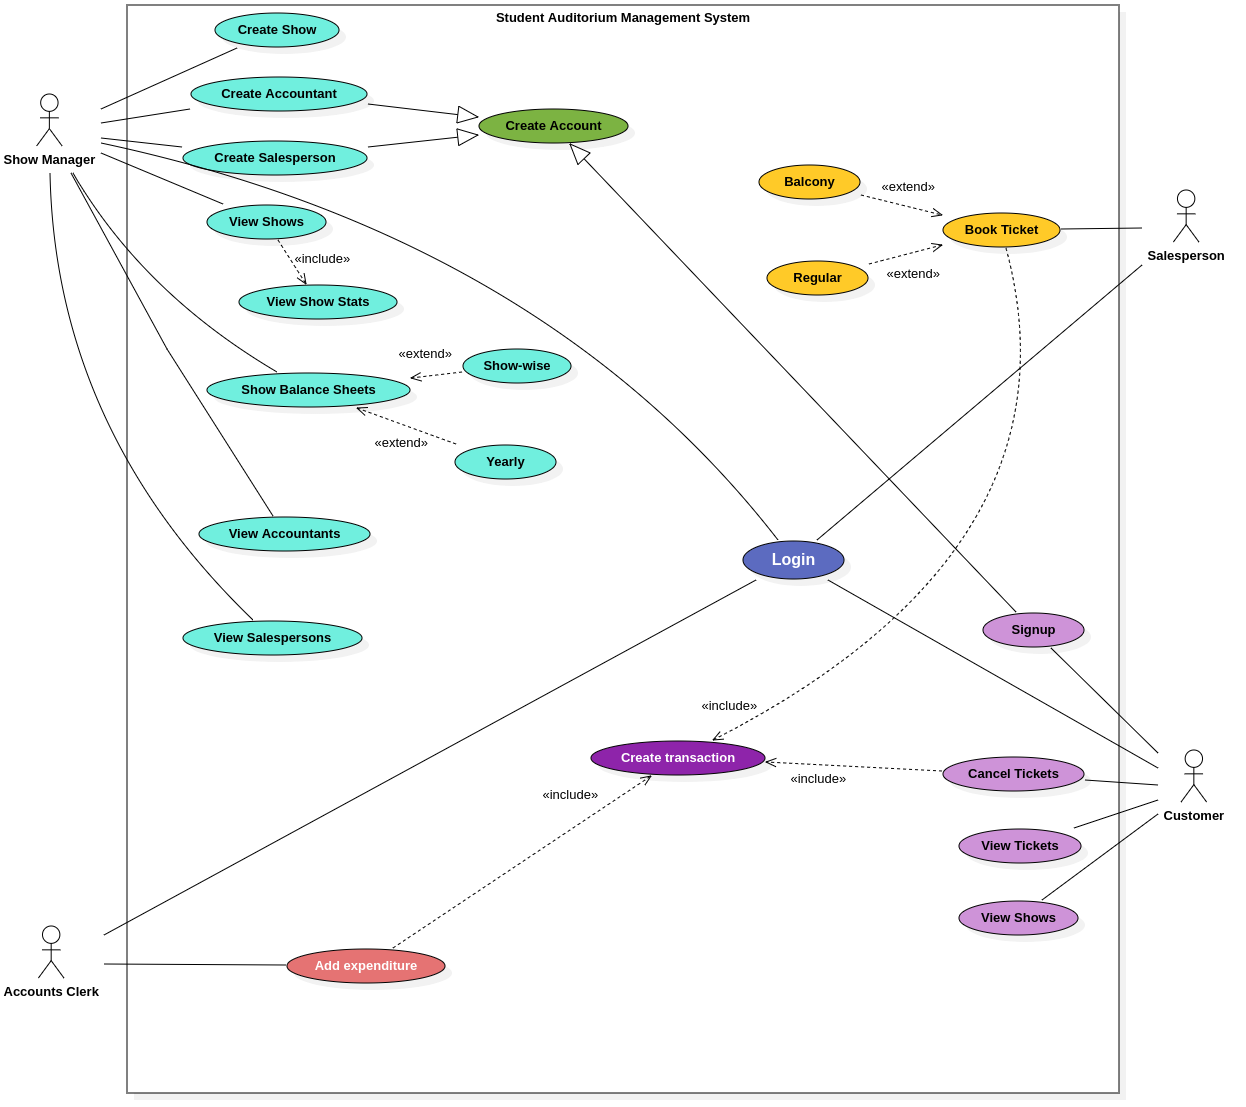
\includegraphics[width=1.3\textwidth]{UseCaseDiagramCrop.png}}
	\caption{Use-Case Diagram for SAMS}
	\label{fig:use-case}
\end{figure}

\section{Appendix C: To Be Determined List}
$<$Collect a numbered list of the TBD (to be determined) references that remain 
in the SRS so they can be tracked to closure.$>$

\end{document}
